\chapter{Электрический заряд. Электрическое поле}
\section{Виды взаимодействий в природе}
    В современной физике выделяют 3 фундаментальных вида взаимодействий:
    ядерное (сильное), электромагнитное и гравитационное. Ниже приводится 
    сравнительная характеристика этих взаимодействий:

    \begin{table}[h]
        \center
        \begin{tabular}[c]{|c|c|c|}\hline
            %-----------------------------------------
            Вид взаимодействия & Отн. величина силы 
            & Радиус действия \\ \hline
            %-----------------------------------------
            Ядерное(сильное) & \(1\) & \(<10^{-15}\) \\ \hline
            
            Электромагнитное & \(10^{-4}\) & \(10^{-15} \ldots \infty\)
            \\ \hline
            
            Гравитационное & \(10^{-40} \ldots 10^{-46}\) & \(\ldots \infty\) 
            \\ \hline
            %-----------------------------------------
        \end{tabular}
    \end{table}
  
\section{Электрический заряд}
    Одним из видов взаимодействий является \textbf{электромагнитное 
    взаимодействие}. Основной его количественной характеристикой является 
    \textbf{электрический заряд}. Перечислим \textit{экспериментально 
    установленные свойства} электрического заряда:
    \begin{figure}[h]
        \center
        \subfigure[Сохранение заряда при поглощении кванта ядром]{
            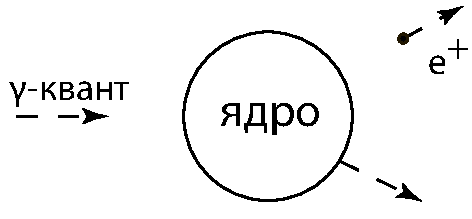
\includegraphics[width=0.47\textwidth]{lec01/save_charge_law_1.pdf}
        }
        \hfill
        \subfigure[Сохранение заряда при аннигиляции]{
            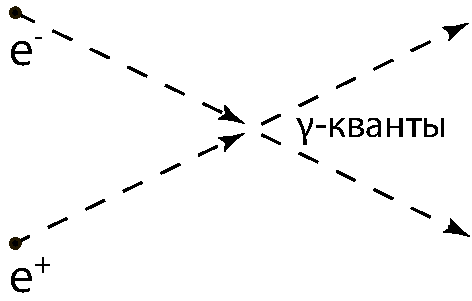
\includegraphics[width=0.47\textwidth]{lec01/save_charge_law_2.pdf}
        }
        \subfigure[Принцип суперпозиции]{
            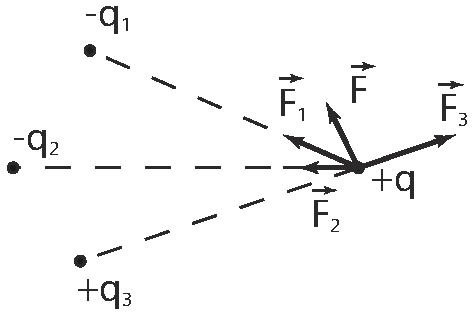
\includegraphics[width=0.47\textwidth]{lec01/superposition.pdf}
        }
        \hfill
        \subfigure[Закон Кулона]{
            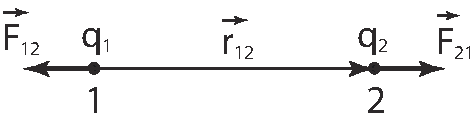
\includegraphics[width=0.47\textwidth]{lec01/coulombs_law.pdf}
        }
        \caption{Свойства электрического заряда}
    \end{figure}
    \begin{enumerate}
    
        \item установлено, что \textbf{существуют 2 сорта зарядов}: заряды, 
        относящиеся к одному из них условно называют положительными, а 
        относящиеся к другому -- отрицательными;
    
        \item установлено, что \textbf{заряды различных сортов притягиваются 
        друг другом, а заряды одного и того же сорта -- отталкиваются};
    
        \item существует \textbf{наименьшая порция электрического заряда}\\ 
        \(e = 1.6~\cdot~10^{-19}~\text{Кл}\) -- заряд электрона;
    
        \item частицы протон и электрон имеют элементарные заряды разных 
        знаков; условились считать заряд протона положительным, а электрона -- 
        отрицательным;
    
        \item \textbf{закон сохранения электрического заряда}: в изолированной 
        системе алгебраическая сумма всех зарядов является постоянной 
        величиной:
        \[
            \sum\pm q_k = \const;
        \]
        
        \item \textbf{принцип суперпозиции}: сила взаимодействия заряда с 
        группой других равна сумме сил взаимодействий этого заряда с каждым 
        зарядом группы;
    
        \item \textbf{закон Кулона}:
        \begin{equation}
            F = k\frac{q_1q_2}{r^2} \label{eq1:1}
        \end{equation}
    
    \end{enumerate}


    В СИ единицей измерения заряда является \textit{Кулон} (Кл). По 
    определению, \( 1\text{Кл} \) -- это заряд переносимый током 
    \( i = 1\text{А} \) за промежуток времени \( \Delta t = 1\text{с} \).
  
    В системе СИ коэффициент \( k \) определяется следующим образом:
    \[
        k = \frac{1}{4\pi\varepsilon_0},
    \]
    где \( \varepsilon_0 = 8,85\cdot10^{-12} \)~ед. СИ -- 
    \textbf{электрическая постоянная}.
  
    Таким образом, в основе электродинамики лежат 3 постулата:
    \begin{enumerate}
        \item закон сохранения заряда;
        \item закон Кулона;
        \item принцип суперпозиции.
    \end{enumerate}


    
    \begin{figure}[h]
        \center
        \subfigure[Определение электрического поля]{
            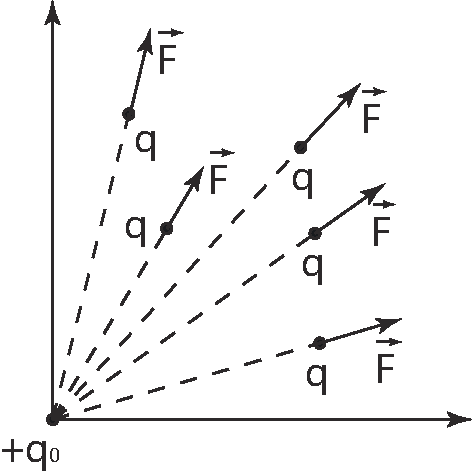
\includegraphics[width=0.30\textwidth]{lec01/electric_field.pdf}
            \label{E_def}
        }
        \hfill
        \subfigure[Напряжённость электрического поля]{
            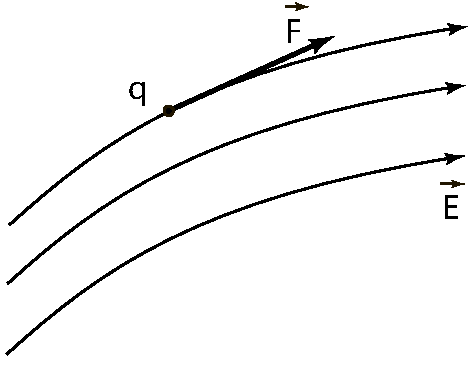
\includegraphics[width=0.30\textwidth]{lec01/E_electric_field.pdf}
        }
        \hfill
        \subfigure[Поле уединённого заряда]{
            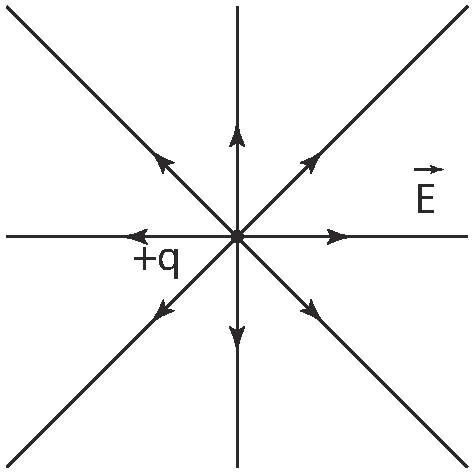
\includegraphics[width=0.30\textwidth]{lec01/field_alone.pdf}
        }
        \hfill
        \subfigure[Поле двух разноимённых зарядов]{
            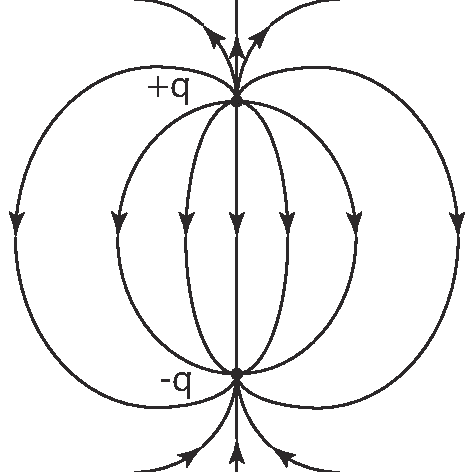
\includegraphics[width=0.47\textwidth]{lec01/field_different.pdf}
        } 
        \hfill
        \subfigure[Поле двух одноимённых зарядов]{
            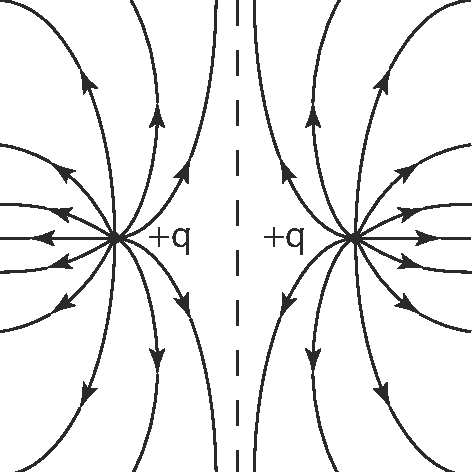
\includegraphics[width=0.47\textwidth]{lec01/field_same.pdf}
        }
        \caption{Электрическое поле}
    \end{figure} 

\section{Электрическое поле}
    Поместим точечный заряд \( q_0 \) в начало координат, а другой точечный 
    заряд \( q \), называемый пробным, будем помещать то в одной, то в другой 
    точке пространства (рис. \ref{E_def}). На заряд в этих точках будет 
    действовать сила
    \[
        \vec{F} = k\frac{q_0q}{r^3}\vec{r}
    \]
    Если в каждой точке пространства определена сила, действующая на единичный 
    пробный заряд, то говорят, что \textit{задано силовое поле}. Так как эта 
    сила имеет электрическое происхождение, то такое силовое поле называется 
    \textbf{электрическим}.
  
    Согласно закону Кулона (\ref{eq1:1}), сила, действующая на точечный заряд 
    \( q \), пропорциональна его величине:
    \begin{equation}
        \vec{F} = \vec{E}q\label{eq1:3}
    \end{equation}

    \begin{definition}
        Физическая величина \( \vec{E} \) называется \textbf{напряженностью 
        электрического поля} и является его основной силовой характеристикой.
    \end{definition}
    \begin{equation}
        \vec{E}=\frac{\vec{F}}{q} \label{eq1:4}
    \end{equation}
    
    Из закона Кулона (\ref{eq1:1}) и определения электрического поля
    (\ref{eq1:3}) следует, что напряжённость электрического поля \( \vec{E} \) 
    выражается следующим образом:
    \begin{equation}
        \vec{E} = \frac{q}{4\pi\varepsilon_0 r^3}\vec{r} \label{eq1:5}
    \end{equation}
  
    \begin{definition}
        Если в некоторой области пространства поле \(\vec{E}\) не зависит от 
        времени, то оно называется \textbf{постоянным}.
    \end{definition}

    В реальной жизни требуется находить напряжённость поля не одного заряда, а 
    группы зарядов. Если мы знаем распределение зарядов в какой-либо области 
    пространства, то при помощи принципа суперпозиции  мы можем узнать какую 
    напряжённость эта группа зарядов создаёт в окружающем пространстве -- 
    определить \textbf{электрическое поле}. Однако, аналитически эту задачу 
    удаётся решить далеко не всегда. Поэтому, обычно, в задачах на вычисление 
    напряжённости рассматриваются симметричные зарядовые конфигурации и 
    специфические области пространства.

    \begin{example}
        Найти напряжённость электрического поля \( \vec{E} \) на оси кольца 
        радиуса \( R \), равномерно заряженного зарядом \( q \).
    \end{example}

    \begin{figure}[b]
        \center
        \subfigure[Равномерно заряженное кольцо]{
            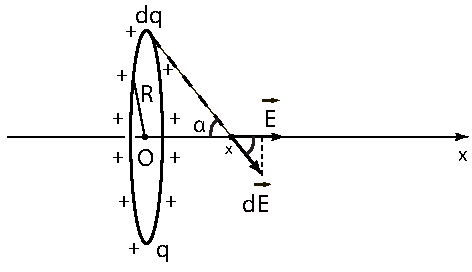
\includegraphics[width=0.47\textwidth]{lec01/ring.pdf}
            \label{1:ring}
        }
        \hfill
        \subfigure[Зависимость \( E(x) \)]{
            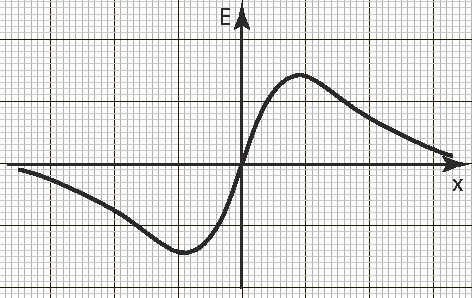
\includegraphics[width=0.47\textwidth]{lec01/E_ring.pdf}
            \label{1:E_ring}
        }
        \caption{К примеру}
    \end{figure}

    \begin{solution}
        Направим вдоль оси кольца ось \( Ox \). В силу симметрии системы, 
        результирующая напряжённость \( \vec{E} \) будет направлена вдоль оси 
        кольца. Разобьём кольцо на малые участки, несущие заряд \( \dd q \).

        Для нахождения напряжённости нужно, воспользовавшись принципом 
        суперпозиции, сложить все проекции на ось \( Ox \) напряжённостей, 
        создаваемых в данной точке \( x \) участками \( \dd q \).

        Проекция \( \dd E_x \) напряжённости поля \( \dd\vec{E} \) на ось
        \( Ox \) может быть найдена следующим образом:
        \[
            \dd E_x = \frac{1}{4\pi\varepsilon_0}\cdot
            \frac{\dd q}{R^2+x^2}\cdot\cos\alpha,
        \]
        где угол \( \alpha \) -- это угол между вектором \( \dd\vec{E} \) и 
        осью \( Ox \). Из треугольника получим
        \[ \cos\alpha = \frac{x}{\sqrt{R^2+x^2}} \].

        Значение \( E \) найдём проинтегрировав по \( q \) выражение для
        \( \dd E_{x} \): 
        \[
            E = \int \dd E_{x} = \frac{x}{4\pi\varepsilon_0\cdot
            (R^2+x^2)^\frac{3}{2}}\cdot\int \dd q = 
            \frac{xq}{4\pi\varepsilon_0\cdot(R^2+x^2)^\frac{3}{2}},
        \]
        или в векторном виде
        \[ 
            \vec{E} = \frac{xq}{4\pi\varepsilon_0\cdot
            (R^2+x^2)^\frac{3}{2}}\cdot\vec{e}_{x}.
        \]

        График этой зависимости изображён на рисунке~\ref{1:E_ring}.
    \end{solution}

